%% abtex2-modelo-slides.tex, v-1.0 gfabinhomat
%% Copyright 2012-2016 by abnTeX2 group at http://www.abntex.net.br/ 
%%
%% This work may be distributed and/or modified under the
%% conditions of the LaTeX Project Public License, either version 1.3
%% of this license or (at your option) any later version.
%% The latest version of this license is in
%%   http://www.latex-project.org/lppl.txt
%% and version 1.3 or later is part of all distributions of LaTeX
%% version 2005/12/01 or later.
%%
%% This work has the LPPL maintenance status `maintained'.
%% 
%% The Current Maintainer of this work is Fábio Rodrigues Silva, 
%% member of abnTeX2 team, led by Lauro César Araujo. 
%% Further information are available on 
%% http://www.abntex.net.br/
%%
%% This work consists of the files abntex2-modelo-slides.tex, 
%% abntex2-modelo-references.bib and abntex2-modelo-marca.pdf
%%
%% Modelo desenvolvido por Fábio Rodrigues Silva (gfabinhomat@gmail.com)
%% Mais informações podem ser obtidas no guia do usuário Beamer 
%% (http://linorg.usp.br/CTAN/macros/latex/contrib/beamer/doc/beameruserguide.pdf)
%% Informações rápidas podem ser acessadas em http://en.wikibooks.org/wiki/LaTeX/Presentations


% Apresentações em widescreen. Outros valores possíveis: 1610, 149, 54, 43 e 32.
% Por padrão, as apresentações são no formato 4:3 (sem o aspectratio).
%\documentclass[aspectratio=169, xcolor=table]{beamer}
\documentclass[aspectratio=169]{beamer}
%[aspectratio=169]
\usetheme{Pittsburgh}
\usecolortheme{default}
\usefonttheme[onlymath]{serif}			% para fontes matemáticas
% Enconte mais temas e cores em http://www.hartwork.org/beamer-theme-matrix/ 
% Veja também http://deic.uab.es/~iblanes/beamer_gallery/index.html

% Customizações de Cores: fg significa cor do texto e bg é cor do fundo
\setbeamercolor{normal text}{fg=black}
\setbeamercolor{alerted text}{fg=red}
\setbeamercolor{author}{fg=blue}
\setbeamercolor{institute}{fg=blue}
\setbeamercolor{date}{fg=green}
\setbeamercolor{frametitle}{fg=red}
\setbeamercolor{framesubtitle}{fg=brown}
\setbeamercolor{block title}{bg=blue, fg=white}		%Cor do título
\setbeamercolor{block body}{bg=gray, fg=darkgray}	%Cor do texto (bg= fundo; fg=texto)

\setbeamertemplate{navigation symbols}{ %\insertslidenavigationsym\\
\insertframenavigationsymbol \insertsubsectionnavigationsymbol \insertsectionnavigationsymbol \insertdocnavigationsymbol \insertbackfindforwardnavigationsymbol \hspace{1em} 	\usebeamerfont{footline}
\insertframenumber/\inserttotalframenumber%
}

% ---
% PACOTES
% ---
\usepackage[alf]{abntex2cite}		% Citações padrão ABNT
\usepackage[english]{babel}		% Idioma do documento
\usepackage{color}			% Controle das cores
\usepackage[T1]{fontenc}		% Selecao de codigos de fonte.
\usepackage{graphicx}			% Inclusão de gráficos
\usepackage[utf8]{inputenc}		% Codificacao do documento (conversão automática dos acentos)
\usepackage{txfonts}			% Fontes virtuais
%\usepackage{listings,bera}
\usepackage[portugues,ruled,lined]{algorithm2e}
\usepackage{algorithmic}
\usepackage{mathtools} % loads amsmath
\usepackage[absolute,overlay]{textpos}
\usepackage{tikz}
\usetikzlibrary{shadows}
%\usepackage[noend]{algpseudocode}
\usepackage{algorithmic}
\setbeamertemplate{caption}[numbered]


\usepackage{listings}
\usepackage{adjustbox}

% ---

% --- Informações do documento ---
\title{Radio Communication to Control and Run an Autonomous Mission for UAVs via a Mobile Application}
\author{Thiago Rodrigo Félix Cavalcante\\Erickson Higor da Silva Alves\\Celso Barbosa de Carvalho}
%\institute{Programa de Pós-Graduação em Engenharia Elétrica
%	    \par
%	    Faculdade de Tecnologia}
\date{Manaus, \today}
% ---

%**
% \PutAt<overlay spec>[<box width>]{(<x>, <y>)}{<content>}
%
% real absolute positioning of <content> on a slide, if content is a figure,
% minipage or whatever kind of LR-box, the <box width> argument may be omitted
%
%
% implementation notes: 
%   - based on   \usepackage[absolute,overlay]{textpos}
%   - NOT combinable with any beamer feature that is based on pgfpages
%     (such as dual-screen support, built-in 2up handouts, etc.), as textpos 
%     and pgfpates interfere at the shippout-level.
%

  \newcommand<>{\PutAt}[3][0pt]{%
    {\only#4{\begin{textblock*}{#1}#2%
      #3
    \end{textblock*}}}%
  }

%**
% \ShowPutAtGrid
%
% draws a helpful grid on the current slide to figure <x> and <y> parameters for \PutAt
% 
  \newcommand{\ShowPutAtGrid}{
    \begin{textblock*}{128mm}(0cm,0cm)
    \tikz[color=red!20!white]\draw[very thin, step=5mm] (0mm,0mm) grid (130mm,100mm);
    \end{textblock*}
    \begin{textblock*}{128mm}(0cm,0cm)
    \begin{tikzpicture}[color=red]
      \draw[step=1cm] (0,0mm) grid (130mm,100mm);   
      \foreach \n in {0,...,12}
        \draw[xshift=.5mm,yshift=-1.5mm, inner sep=0pt, anchor=west] (\n,10) node {\scriptsize{\textbf{\n}}};
      \foreach \n in {1,...,9}
        \draw[xshift=.5mm,yshift=-1.5mm, inner sep=0pt, anchor=west] (0,10-\n) node {\scriptsize{\textbf{\n}}};
    \end{tikzpicture}
    \end{textblock*}
  }


%**
% \NormalBox<overlay spec>[tikz picture/node options]{<content>}
%
% draws content boxed in a nice box
% 
\newcommand<>{\NormalBox}[2][]{%
  \only#3{\tikz[#1, every node/.style={shape=rectangle,draw,fill=white, drop shadow, #1}]\node []{#2};}
}
%**
% \OrangeBox<overlay spec>[tikz picture/node options]{<content>}
%
% draws content boxed in an orange call-out box
% 
\newcommand<>{\OrangeBox}[2][]{%
  \onslide#3{\NormalBox[fill=orange!30,draw=black!30,rounded corners=4pt,#1]{#2}}%
}


% ----------------- INÍCIO DO DOCUMENTO --------------------------------------
\begin{document}

% ----------------- NOVO SLIDE --------------------------------
\begin{frame}

\begin{minipage}{1\linewidth}
  \centering
  \begin{tabular}{cc}
    \begin{tabular}{c}
      
\includegraphics[scale=0.1]{ufam.eps}
    \end{tabular}
    &
    \begin{tabular}{c}
      \textbf{Universidade Federal do Amazonas} \\ \textbf{Faculdade de Tecnologia}
    \end{tabular}
  \end{tabular}
\end{minipage}

\titlepage

\end{frame}

% ----------------- NOVO SLIDE --------------------------------
\begin{frame}{Contents}
\tableofcontents
\end{frame}


% ----------------- NOVO SLIDE --------------------------------
\section{Introduction}

\begin{frame}{Introduction}

Logistics has become a competitive and fundamental factor for organizations, involving the management, conservation, and supervision of freight transport. In addition, excellent logistics means client satisfaction; so speed is still an important factor in a successful logistics process~\cite{drone4logistic}.

\end{frame}
\begin{frame}{Introduction}

In this work we present a methodology to carry out a mission, \textit{i.e.}, a client order, in a production environment. Such mission is previously planned, so that the distance travelled by the UAV is optimized. Moreover, these components are implemented in an Android application, which uses radio waves to communicate with the drone. The mobile app is useful for leaders and/or managers, since they are able to supervise production lines in real-time, checking statuses and acting on failures.

\end{frame}

\section{Methodology}
\begin{frame}{Methodology}
\frametitle{Methodology}
\framesubtitle{Functioning Diagram}\pause

 \begin{figure}[H]
  \centering
  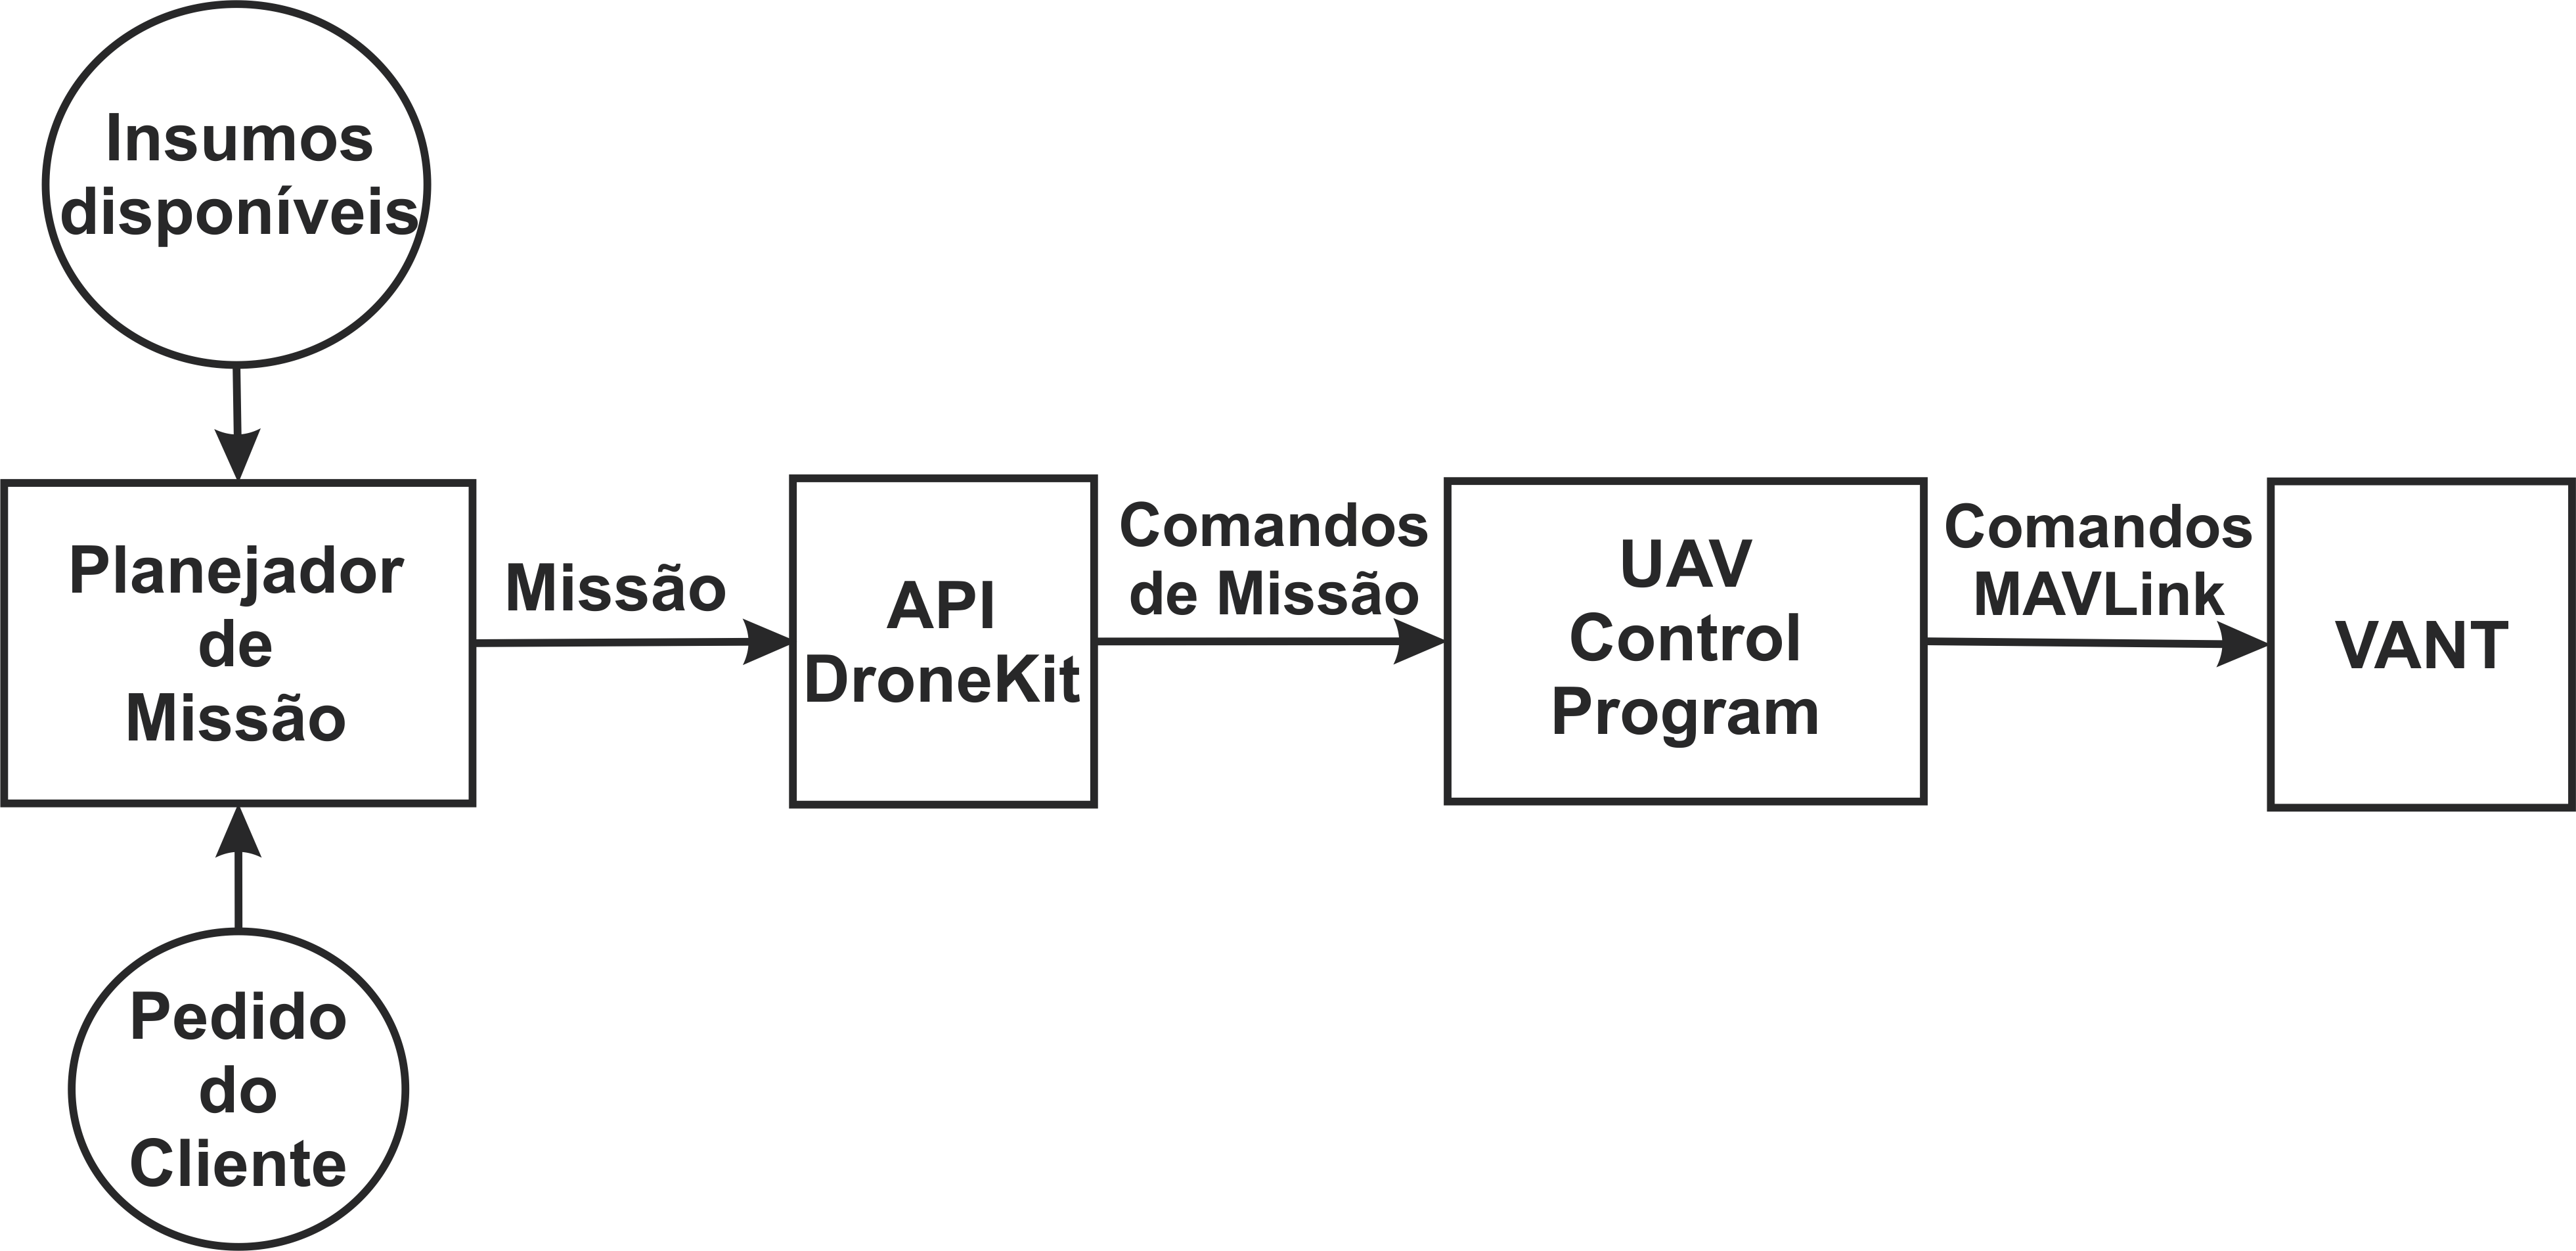
\includegraphics[scale=0.4]{sysArchAndPort.eps}
  %\caption{Diagram}
\end{figure}

\end{frame}

\begin{frame}{Methodology}
\frametitle{Methodology}
\framesubtitle{Use Case Environment}\pause

 \begin{figure}[H]
  \centering
  \includegraphics[scale=0.55]{useCase.eps}
  %\caption{Diagram}
 \end{figure}

\end{frame}

\section{Results}
\begin{frame}{Results}
\frametitle{Results} 	
%\framesubtitle{Sketching}
\pause

\begin{table}[H]
\centering
\caption{Mission Flight Time Tested in Real and Virtual UAV.}
\begin{tabular}{c|c|c|}
\cline{2-3}
\textbf{}                                     & \textbf{Real UAV}                 & \textbf{Virtual UAV}              \\ \hline
\multicolumn{1}{|c|}{\textit{\textbf{Tests}}} & \textit{\textbf{Flight Time (s)}} & \textit{\textbf{Flight Time (s)}} \\ \hline
\multicolumn{1}{|c|}{1}                       & 441.720                           & 430.830                           \\ \hline
\multicolumn{1}{|c|}{2}                       & 440.180                           & 436.885                           \\ \hline
\multicolumn{1}{|c|}{3}                       & 447.510                           & 441.681                           \\ \hline
\multicolumn{1}{|c|}{4}                       & 438.190                           & 441.227                           \\ \hline
\multicolumn{1}{|c|}{5}                       & 445.850                           & 451.865                           \\ \hline
\end{tabular}
\label{table:tests}
\end{table}

\end{frame}

\section{Conclusions}
\begin{frame}{Conclusions}
\frametitle{Conclusions}\pause

\begin{itemize}
\item we have developed an Android application to supervise production status and allow real-time monitoring for line managers/leaders;\pause

\item we have developed a framework for mission planning, command and control for intralogistics mission using a commercial UAV. We used an UAV to solve intralogistics problems using the DroneKit API to control and command adopting a high-level programming language.
\end{itemize}

\end{frame}

\section{Critique}
\begin{frame}{Critique}
\frametitle{Critique}\pause

\begin{itemize}
\item the use of computational vision for the recognition of inputs, and improvements of the UAV system used;\pause
\item evaluate the communication between the drone and the application using different frameworks/protocols, in order to improve the supervision step.
\end{itemize}

\end{frame}

% ----------------- NOVO SLIDE --------------------------------
\section{References}

% --- O comando \allowframebreaks ---
% Se o conteúdo não se encaixa em um quadro, a opção allowframebreaks instrui 
% beamer para quebrá-lo automaticamente entre dois ou mais quadros,
% mantendo o frametitle do primeiro quadro (dado como argumento) e acrescentando 
% um número romano ou algo parecido na continuação.

\begin{frame}[allowframebreaks]{References}
\bibliography{ref-slides}
\end{frame}

% ----------------- FIM DO DOCUMENTO -----------------------------------------
\end{document}
